\subsection{pbdMPI Example: Random Forest Prediction}
\makesubcontentsslidessec


\begin{frame}[fragile]{Letter Recognition Data}
  \begin{exampleblock}{Example \countex : Letter Recognition data from
      package \pkg{mlbench} (20,000 $\times$ 17)}\pause
    \vspace{-1em}
    \begin{minipage}{0.3\textwidth}
      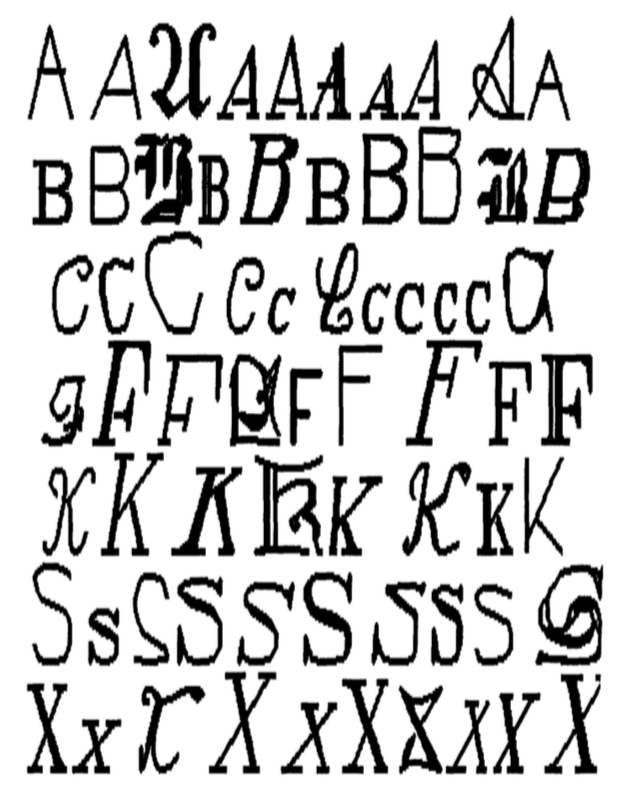
\includegraphics[width=0.95\textwidth]{../common/pics/apps/ML_FreySlate1991}
    \end{minipage}
    \begin{minipage}{0.69\textwidth}\tiny
      \begin{lstlisting}
[,1]	lettr	capital letter
[,2]	x.box	horizontal position of box
[,3]	y.box	vertical position of box
[,4]	width	width of box
[,5]	high	height of box
[,6]	onpix	total number of on pixels
[,7]	x.bar	mean x of on pixels in box
[,8]	y.bar	mean y of on pixels in box
[,9]	x2bar	mean x variance
[,10]	y2bar	mean y variance
[,11]	xybar	mean x y correlation
[,12]	x2ybr	mean of x^2 y
[,13]	xy2br	mean of x y^2
[,14]	x.ege	mean edge count left to right
[,15]	xegvy	correlation of x.ege with y
[,16]	y.ege	mean edge count bottom to top
[,17]	yegvx	correlation of y.ege with x
      \end{lstlisting}
    \end{minipage} \\
    {\tiny P. W. Frey and D. J. Slate (Machine Learning Vol 6/2 March 91):
    "Letter Recognition Using Holland-style Adaptive Classifiers".}
  \end{exampleblock}
\end{frame}


\begin{frame}
  \begin{exampleblock}{Example \showex : Random Forest Algorithm}\pause
    \begin{enumerate}
     \item Build simple regression trees from random subsets of
       columns
     \item Use model averaging for prediction
     \item Package \pkg{randomForest} has a \code{combine()} function
       that enables the following parallel approach:
       \begin{enumerate}
       \item Everyone gets the same training data
       \item Split regression tree building among processors
         (\pkg{randomForest})
       \item Use \code{allgather} to bring built predictors to all
       \item Everyone \code{combine} predictors
       \item Split prediction work by blocks of rows
       \item Use \code{allreduce} to assess prediction
       \end{enumerate}
     \item Steps (3) and (4) can be improved with a custom
       reduce/combine to take advantage of MPI vendor optimizations
    \end{enumerate}
  \end{exampleblock}
\end{frame}


\begin{frame}[fragile]
  \begin{exampleblock}{Example \showex :  Random Forest Code \\
      (Split learning by blocks of trees. Split prediction by blocks
      of rows.)}\pause
    \begin{lstlisting}[title=Serial Code]
data(LetterRecognition) # 26 Capital Letters Data 20,000 x 17
set.seed(seed=1234567)
n <- nrow(LetterRecognition)
## get train data
n_train <- floor(0.8*n)
i_train <- sample.int(n, n_train) # Use 4/5 of the data to train
train <- LetterRecognition[i_train, ]
test <- LetterRecognition[-i_train, ]

## train random forest
my.k <- 500
rf.all <- randomForest(lettr ~ ., train, ntree=my.k, norm.votes=FALSE)

## predict test data
pred <- predict(rf.all, test)
correct <- sum(pred == test$lettr)
cat("Proportion Correct:", correct/(n - n_train), "\n")
    \end{lstlisting} %$
  \end{exampleblock}
\end{frame}


\begin{frame}[fragile]
  \begin{exampleblock}{Example \showex :  Random Forest Code \\
      (Split learning by blocks of trees. Split prediction by blocks
      of rows.)}\pause
    \begin{lstlisting}[title=Parallel Code,escapeinside={(*@}{@*)}]
data(LetterRecognition) # 26 Capital Letters Data 20,000 x 17
(*@\textcolor{red}{comm.}@*)set.seed(seed=123(*@\textcolor{red}{, diff=FALSE}@*)) # same training data
n <- nrow(LetterRecognition)
n_train <- floor(0.8*n)
i_train <- sample.int(n, n_train) # Use 4/5 of the data to train
train <- LetterRecognition[i_train, ]
(*@\textcolor{red}{my.test\_rows <- get.jid(n - n\_train)}@*)  # different test data
test <- LetterRecognition[-i_train, ](*@\textcolor{red}{[my.test\_rows, ]}@*)

(*@\textcolor{red}{comm.}@*)set.seed(seed=1e6*runif(1)(*@\textcolor{red}{, diff=TRUE}@*))
my.k <- floor(500(*@\textcolor{red}{/comm.size()}@*))
my.rf <- randomForest(lettr ~ ., train, ntree=my.k, norm.votes=FALSE)

(*@\textcolor{red}{rf.each <- allgather(my.rf)}@*)
(*@\textcolor{red}{rf.all <- do.call(combine, rf.each)}@*)

pred <- predict(rf.all, test)
correct <- (*@\textcolor{red}{allreduce(}@*)sum(pred == test\$lettr)(*@\textcolor{red}{)}@*)
(*@\textcolor{red}{comm.}@*)cat("Proportion Correct:", correct/(n - n_train), "\n")
    \end{lstlisting} %$
  \end{exampleblock}
\end{frame}